\documentclass[11pt]{article}

\usepackage[margin=1in]{geometry}
\usepackage{hyperref}
\usepackage{url}
\usepackage{booktabs}
\usepackage{amsmath,amssymb}
\usepackage{enumitem}
\usepackage{graphicx}
\usepackage{xcolor}
\usepackage{array}
\usepackage{tikz}
\usepackage{longtable}

\usetikzlibrary{arrows.meta,positioning,fit,backgrounds,calc}

\definecolor{layerblue}{RGB}{62,112,191}
\definecolor{layergreen}{RGB}{73,151,105}
\definecolor{layerorange}{RGB}{214,126,44}
\definecolor{layerred}{RGB}{188,76,76}
\definecolor{layergray}{RGB}{92,99,112}

\title{CivStation: Technical Report on an Experimental Layered Stack for Civilization VI Computer Use}
\author{Minsing Jin}
\date{March 26, 2026}

\begin{document}
\maketitle

\begin{abstract}
This technical report documents CivStation, an experimental software stack for building, steering, and instrumenting Civilization VI computer-use agents. The project does not yet constitute a validated benchmark suite, a robust long-running agent, or a completed empirical research artifact. Instead, it should be read as an engineering workbench and design record that explores how to structure long-horizon game control around explicit context, strategy, action, and human-in-the-loop layers. The report summarizes the architecture, control surfaces, normalization scheme for screen actions, exploratory VLM trade-off instrumentation, the reasons the current system has not yet produced stable long-running experimental results, and the directions that would need to mature before stronger research claims become justified. The purpose is to preserve technical lessons and make future iterations easier to design, audit, and extend.
\end{abstract}

\section{Status Note}

This document is best understood as a \emph{technical report}, not as a benchmark paper or a result-focused systems paper. The current stack is useful as experimental infrastructure and as a record of design choices, failure modes, and future directions. It is not yet the right basis for strong claims about benchmark maturity or long-running autonomous game performance.

\section{Purpose}

The purpose of CivStation is to act as an experimental stack for studying long-horizon computer use in a turn-based strategy game. The motivation is straightforward: a game like Civilization VI exposes many of the difficulties that also appear in real computer-use systems, including partial observability, changing interface modes, delayed consequences, brittle action execution, and the need for operator intervention.

The current value of the project is infrastructural rather than empirical. CivStation is useful as a technical base for future work on live agent evaluation, human-versus-agent comparison, HITL-versus-autonomous comparisons, and agent-versus-agent matches. It is not yet a completed benchmark suite, and it is not yet a robust long-running game-playing agent. The right claim today is therefore modest: CivStation is a structured experimental stack that makes future benchmark work more plausible, while also making current limitations easier to inspect.

\section{System Overview}

CivStation decomposes the runtime into four explicit layers:
\begin{itemize}[leftmargin=*]
    \item \textbf{Context}: what the system believes about the current game state
    \item \textbf{Strategy}: what should matter next given state and human intent
    \item \textbf{Action}: which primitive should handle the screen and what action to take
    \item \textbf{HitL}: how a human supervises, interrupts, or redirects the run
\end{itemize}

This separation is the main architectural idea in the project. The system is deliberately not presented as a single prompt loop.

\begin{figure}[h]
    \centering
    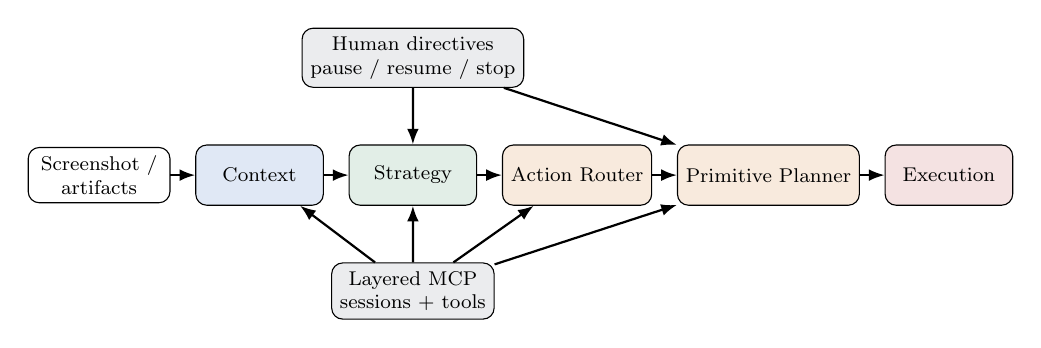
\begin{tikzpicture}[
        scale=0.9,
        transform shape,
        node distance=0.35cm and 0.35cm,
        box/.style={draw, rounded corners, align=center, minimum width=2.0cm, minimum height=0.78cm, font=\footnotesize, fill=white},
        side/.style={draw, rounded corners, align=center, minimum width=2.1cm, minimum height=0.78cm, font=\footnotesize, fill=layergray!12},
        contextbox/.style={draw, rounded corners, align=center, minimum width=1.8cm, minimum height=0.85cm, font=\footnotesize, fill=layerblue!16},
        strategybox/.style={draw, rounded corners, align=center, minimum width=1.8cm, minimum height=0.85cm, font=\footnotesize, fill=layergreen!16},
        actionbox/.style={draw, rounded corners, align=center, minimum width=1.8cm, minimum height=0.85cm, font=\footnotesize, fill=layerorange!16},
        execbox/.style={draw, rounded corners, align=center, minimum width=1.8cm, minimum height=0.85cm, font=\footnotesize, fill=layerred!16},
        arr/.style={-{Latex[length=2mm]}, thick}
    ]
    \node[box] (capture) {Screenshot /\\artifacts};
    \node[contextbox, right=of capture] (context) {Context};
    \node[strategybox, right=of context] (strategy) {Strategy};
    \node[actionbox, right=of strategy] (router) {Action Router};
    \node[actionbox, right=of router] (primitive) {Primitive Planner};
    \node[execbox, right=of primitive] (execute) {Execution};

    \node[side, above=0.8cm of strategy] (human) {Human directives\\pause / resume / stop};
    \node[side, below=0.8cm of strategy] (mcp) {Layered MCP\\sessions + tools};

    \draw[arr] (capture) -- (context);
    \draw[arr] (context) -- (strategy);
    \draw[arr] (strategy) -- (router);
    \draw[arr] (router) -- (primitive);
    \draw[arr] (primitive) -- (execute);
    \draw[arr] (human) -- (strategy);
    \draw[arr] (human) -- (primitive);
    \draw[arr] (mcp) -- (context);
    \draw[arr] (mcp) -- (strategy);
    \draw[arr] (mcp) -- (router);
    \draw[arr] (mcp) -- (primitive);
    \end{tikzpicture}
    \caption{Layered runtime view of CivStation.}
\end{figure}

\section{Action Representation}

One practical design choice is to ask the model to emit actions in a normalized coordinate space rather than in raw monitor coordinates. The runtime then restores those normalized coordinates into the actual monitor or game-window resolution before execution. This makes it possible to:
\begin{itemize}[leftmargin=*]
    \item decouple prompts from local display resolution
    \item support cropped game-window execution
    \item reduce the coupling between model output and platform-specific screen geometry
\end{itemize}

This normalization-and-restore mechanism is one of the few genuinely reusable components in the project and remains useful even if the higher-level benchmarking story changes.

\section{Control and Instrumentation}

The stack includes:
\begin{itemize}[leftmargin=*]
    \item a local dashboard
    \item REST and WebSocket control
    \item a layered MCP server
    \item primitive-specific multi-step flows
    \item fallback and semantic verification hooks
    \item image-preprocessing and latency/quality instrumentation
\end{itemize}

This makes CivStation more valuable as an experimental workbench than as a finished autonomous system.

\section{What Was Explored}

The repository contains exploratory work on several questions:
\begin{itemize}[leftmargin=*]
    \item how image downscaling and compression affect VLM latency
    \item how contrast and color policies affect action extraction
    \item how provider/model choice changes synthetic action behavior
    \item how fallback and semantic verification might work in multi-step UI flows
\end{itemize}

These explorations are recorded as engineering artifacts rather than as definitive benchmark results. They are valuable mainly because they expose practical bottlenecks that would otherwise remain anecdotal.

\section{Current Limitations}

The most important limitation is that the project has not yet produced stable long-running Civilization VI experiments. In practice:
\begin{itemize}[leftmargin=*]
    \item a human must usually launch and maintain the live game session
    \item slow inference can make the system too sluggish for reliable interaction
    \item interruption, modal events, and state drift can break runs
    \item fallback logic is hard because action verification often depends on the same imperfect VLM stack
    \item repeated bugs and brittle edge cases prevent clean experiment loops
\end{itemize}

For these reasons, the project should not currently be represented as a validated benchmark or as a finished research system. At most, it should be represented as an experimental stack that preserves architectural ideas and empirical lessons for later work.

\section{Why It Is Still Worth Keeping}

Even without successful experiments, the project still has value as a technical record. It captures:
\begin{itemize}[leftmargin=*]
    \item one concrete layered architecture for long-horizon game computer use
    \item explicit lessons about why long-running VLM-only control is hard
    \item practical infrastructure for future HITL and benchmark-oriented work
    \item reusable components such as action normalization, layered control, and MCP exposure
\end{itemize}

That makes it worth keeping as a technical report, even if it is not yet worth presenting as a paper with strong empirical claims. The main value is not in proving that the approach already works. The value is in preserving the engineering decomposition, the failure boundaries, and the practical lessons about what must be solved next.

\section{Future Directions}

The most realistic future directions are:
\begin{itemize}[leftmargin=*]
    \item stabilize long-running execution before claiming benchmark value
    \item improve verification and fallback logic
    \item explore hybrid architectures where VLMs perform visual understanding and faster models or native-app-specific VLAs handle micro-actions
    \item eventually evaluate live modes such as human vs agent, agent vs agent, and HITL vs autonomous
\end{itemize}

\section{Artifact Locations}

All paper-related materials are grouped under \texttt{docs/paper/}. Experimental artifacts are under \texttt{docs/paper/arxiv/results/}, and paper-specific scripts are under \texttt{docs/paper/scripts/}.

\section{Recommended Public Use}

If only one document from this repository is publicly archived, this technical report should be the default choice. It is the most accurate and least overstated representation of the current state of the project. The companion research memo is also useful, but primarily as a failure-oriented supplement.

\end{document}
